\chapter{绪论}

\section{引言}
子痫前期(preeclampsia, PE)又作先兆子痫,是孕妇妊娠期特有的一种多系统进展性疾病, 与妊娠期高血压(gestational hypertension)、子痫(eclampsia)、
慢性高血压并发子痫前期(chronic hypertension with superimposed preeclampsia)以及妊娠合并慢性高血压(chronic hypertension)统称妊娠期
高血压疾病(hypertension disorders of pregnancy, HDP)\cite{OAG9,HDASOM,2000s1}。
子痫前期临床表现的显著特点是原发性高血压与蛋白尿。
近年来,组织的对子痫前期的涵盖范围进行了进一步的拓展,在妊娠20周后出现新发(原发)高血压,在两次间隔$4h$或$4h$以上的血压测定中,收缩压≥$140mmHg$和(或)
舒张压≥$90mmHg$,且伴有下列任一项或多项\cite{OAG9,FIGO}:
\begin{itemize}
    \item 孕妇出现蛋白尿症状,尿蛋白≥$300mg/24h$,或尿蛋白/肌酸酐比值≥$30mg/mol$,或随机尿蛋白≥(+);
    \item 孕妇无尿蛋白但伴有以下任一器官或系统功能紊乱、受累受损:心、肺(肺水肿)、肝(血清转氨酶水平为正常值2倍以上)、肾(血肌酐水平大于$1.1mg/dl$
    或为正常值2倍以上)等重要器官,或血液系统(血小板<$100 \times 10^{9}/L$)等)、消化系统、神经系统的异常改变等;
    \item 胎盘-胎儿受到累及:胎盘胎儿生长受限、脐动脉多普勒分析检测异常、死胎等。 
\end{itemize}

妊娠期高血压疾病可引起严重的母胎并发症,是孕产妇和围产儿病死率升高的主要原因\cite{OAG9}。
据世界卫生组织统计,子痫前期在孕妇中发病率高达5\%-10\%,是除体内大出血外孕妇死亡的第二大危险因素\cite{LCT2006},每年可导致全球范围内约76 000名孕妇死亡,并进一步导致约500 000
名胎儿/婴儿的死亡\cite{DAM2015,LCT2006}(如\autoref{fig:dhd}所示)。为推广普及人们对危及母婴生命安全的子痫前期的认知,同时教育女性了解她们当前及长期的健康风险,
全球孕妇保健组织自2017年起将每年的5月22日确定为世界子痫日(world preeclampsia day)(如\autoref{fig:wpd}所示)。
\begin{figure}[h]
    \centering
    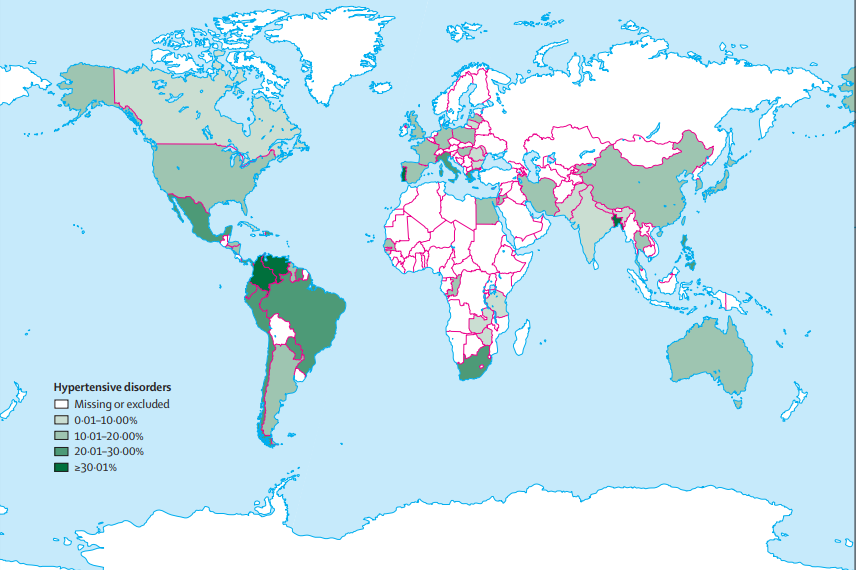
\includegraphics[width=.7\linewidth]{ch1/dhd}
    \caption{\label{fig:dhd}因妊娠期高血压疾病死亡孕妇的国家分布比例}
\end{figure}
\begin{figure}[h]
    \centering
    
\includegraphics[width=.7\linewidth]{ch1/wpd}
    \caption{\label{fig:wpd}2021年世界子痫日主题:Preeclampsia: Beyond Pregnancy}
\end{figure}

就现阶段我国国情而言,由于人口基数大、人口出生率较高,导致每年妊娠孕妇数及新生儿数总量大。
同时,自全面开放二孩政策后,各地区高龄孕妇、二次妊娠孕妇比例明显提升。而临床研究已经证实,
高龄与二(三)次妊娠均属于可能导致子痫前期的风险因素,会增加孕妇子痫前期的患病可能。

因此,如何对子痫前期快速有效的医学诊断与干预成为新的难题,实现子痫前期的预测和及早诊断,
是对孕妇子痫前期的治疗及孕妇、围生儿的健康安全的保障,具有重大的临床应用价值。
\section{子痫前期的病理及危害}
\subsection{病因及发病机制}
截止目前,医学界对子痫前期的病因与发病机制尚未完全明确,相关研究还在继续进行之中。但得到公认的一点是,子痫前期病发具有异质性,多因素、多机制及多通路均对子痫前期的发病有所影响,不能仅以“一元论”的观点对待。
目前临床对子痫前期的病因和发病机制的主要有以下几种学说:

一、子宫螺旋小动脉重铸不足

该学说认为子痫前期的发病与妊娠早期胎盘功能紊乱密切相关\cite{OAG9,Duvekot2010},其作用机制可以概括为两个阶段,如\autoref{fig:ppp}所示。
在第一阶段,孕妇子宫螺旋动脉重构受损、出现重铸障碍,绒毛外滋养细胞浸润能力受损,导致胎盘缺血、缺氧,释放多种胎盘因子,该阶段无明显临床现象;在第二阶段,各种胎盘因子进入母体血液循环,血管阻力增大,胎盘灌注减少,
促进系统性炎症反应的激活及血管内皮损伤引起子痫前期-子痫多样化的临床表现。尽管造成子宫螺旋小动脉重铸足的机制尚待研究,该学说是目前临床最为普遍接受的。
\begin{figure}[htbp]
    \centering
    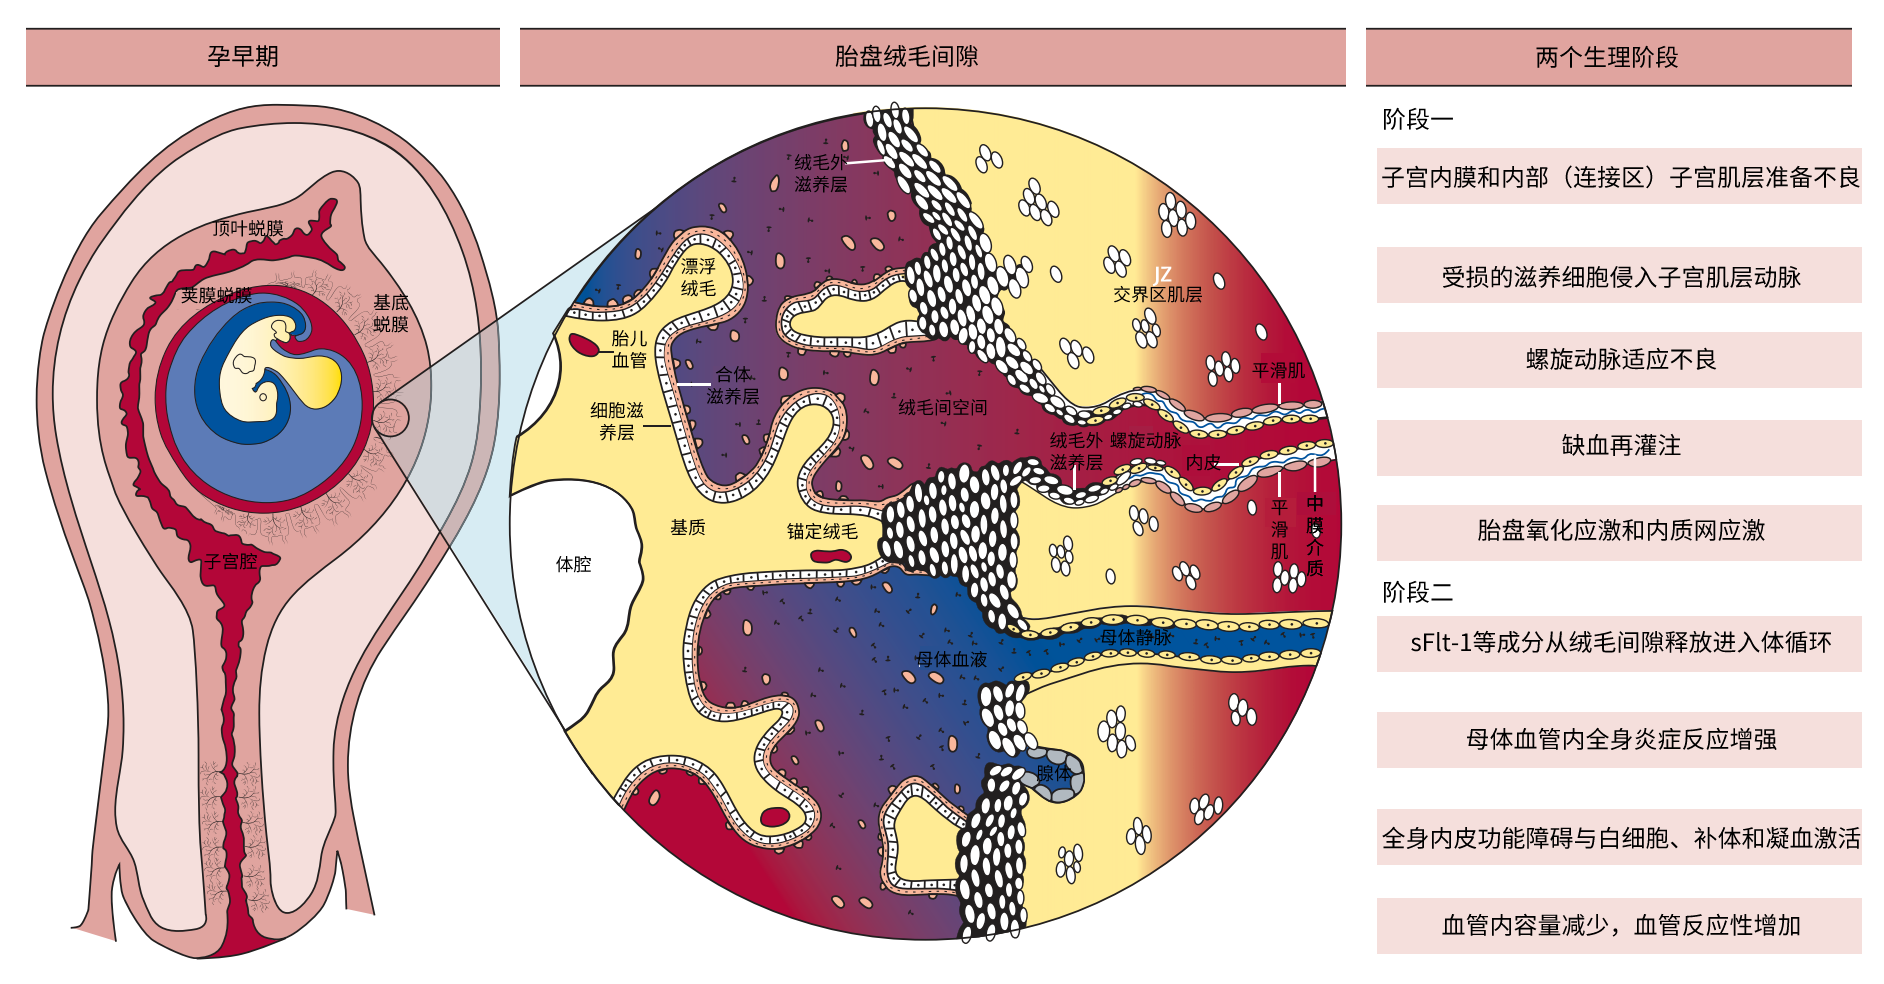
\includegraphics[width=.7\linewidth]{ch1/ppp}
    \caption{\label{fig:ppp}一种子痫前期可能的发病机制}
\end{figure}

二、炎症免疫过度激活

该学说认为子痫前期是母系-父系免疫适应不良导致的\cite{Sibai2005,OAG9,Shi2006},即胎儿胎盘具有的半抗原性移植体特性导致同种异体移植排斥,最终引起的母系同种免疫反应从而诱发子痫前期。
精子内有组织相容性的白细胞分化抗原(HLA)存在,很多学者已发现当母体滋养细胞不能够表达足够强的移植物抗原(HLA-A, HLA-B, HLA-D)\cite{Moffett2002}时,母体T细胞是无法识别HLA的,
从而使母体对胚胎免疫耐受降低。妊高征患者HLA抗体的检出率明显高于正常孕妇、妊高征患者体液免疫与细胞免疫功能异常等临床现象都能与免疫学说较好的验证。

三、血管内皮细胞损伤及前列腺素合成失调

该观点认为,当血管内皮细胞出现损伤后,将进一步导致前列腺素合成失调\cite{OAG9,Sibai2005}。它使扩血管物质如一氧化氮(NO)、前列环素(PGI2),合成减少,而缩血管物质如内皮素(ET)、血栓索(TXA2)等合成增加,从而促进血管痉挛。
此外血管内皮损伤还可使抗凝血酶(ATⅢ)减少并激活血小板及凝血因子进入母体血循环,导致凝血功能增加,纤溶活性抑制,加之血管痉挛,内皮细胞损伤,胶原暴露,激发血管内凝血,甚至是血栓的出现。

四、遗传因素

子痫前期具有家族倾向性,提示遗传因素与该病发生有关\cite{OAG9,Sibai2005}。临床研究发现子痫前期主要体现为母系遗传,家系分析发现\cite{Ge2013},妊高征患者一级亲
属及二级亲属的发病率比无家族史孕妇明显增高,这表明孕妇对妊高征有遗传易患性,且目前多倾向于多基因遗传,其具体的遗传规律目前尚有争议。由于子痫前期的异质性,尤其是遗传
和环境因素的交互作用产生了复杂的表型。在子痫前期遗传易感性研究中,尽管目前已定位了十几个子痛前期染色体易感区域,但在该区域内进一步寻找易感基因仍面临很大的挑战。

五、其他学说

近几年来,学者们还相继提出一些新的可能引起子痫前期的学术观点,如胎盘因子学说\cite{Shi2006}等。同时一些临床研究也发现,多种营养因素如低白蛋白血症、钙、镁、锌、硒等缺乏与子痫前期发生发展
可能有关\cite{OAG9}。但此类学说与假设仍需进一步临床研究与理论研究来证实。

\subsection{子痫前期引起的生理变化及危害}
子痫前期引起的基本的病理生理变化是全身小动脉痉挛、血管内皮损伤和水钠潴留。全身各脏器各系统灌注减少,对母儿造成危害,甚至导致母儿死亡。由于该病表现为多脏器和系统损害,故有学者提出子痫前期
-子痫综合征(preeclampsia-eclampsia syndrome)的概念。

一、全身小动脉痉挛 

可能由于升压系统和降压系统平衡失调,血管壁对某些升压物质(如血管紧张素Ⅱ)的反应性增强,从而使全身小动脉,特别是直径200um以下的小动脉发生痉挛,导致各器官供血不足,外周阻力增高,产生高血压等一系列症状体征。

子宫血管痉挛,胎盘供血不足,绒毛退行性变、出血、坏死、梗塞等,导致胎盘提高老化,功能不全。病变进行缓慢时,可致胎儿宫内生长发育迟缓(IUGR),病变急剧时,可致胎死宫内,严重时胎盘后小血管破裂,导致胎盘早剥。

脑部血管痉挛,脑组织缺氧、水肿、严重时出血,出现头昏、头痛、恶心、呕吐,重者抽搐、昏迷,脑疝形成而致死亡。

心脏血管痉挛,心肌缺血、间质水肿、点状出血及坏死,加之血液粘稠度增加,外周阻力增加,心脏负担加重,可导致左心衰竭,继而发生肺水肿。

肾脏血管痉挛,肾血流量减少,组织缺氧,血管壁通透性增加,血浆从肾小球漏出,出现蛋白尿及管型。肾小球毛细血管痉挛,肾小球内皮细胞肿胀,发生血管内凝血,纤维蛋白沉着,肾小球滤过率减少,出现尿少,严重者出现肾功衰竭。

肝脏由于缺血,肝细胞线粒体内所含的谷丙转氨酶释放,可致血清谷丙转氨酶升高,出现黄疸表明病情严重。肝脏主要病变为门静脉周围有局限性出血,继而纤维素性血栓形成,严重者肝实质缺血坏死、肝包膜下出血。

眼底小动脉痉挛、缺血、水肿,严重时渗出、出血,甚至视网膜剥离,出现眼花、视物模糊,甚至失明。

二、水钠潴留 

可能由于肾小球滤过率减少,肾小管对钠的重吸收增加,钠离子潴留细胞外而引起水肿。肾上腺皮质激素、抗利尿激素分泌增加,也可能是水潴留的另一个原因。由于水钠潴留,组织水肿,体重异常增加。

\section{子痫前期的研究现状}
现代医学对子痫前期的认知经历了漫长的探索\cite{BJOG2016}。

下面将以临床对子痫前期发生评估的各项检测参数、检测设备及新兴检测技术三方面进行介绍。
\subsection{检测参数}
一、风险因子

已有研究表明,许多孕妇自身风险因子与子痫前期的发生密切相关\cite{Magee2008,FIGO,Lowe2015,Heazell2010}。临床医生往往会以量表问卷的形式向孕妇采集这些信息,
对孕妇罹患子痫前期的可能进行初筛\cite{risks},如\autoref{fig:risk}所示。常见的子痫前期风险因子包含以下几点:
\begin{figure}[htbp]
    \centering
    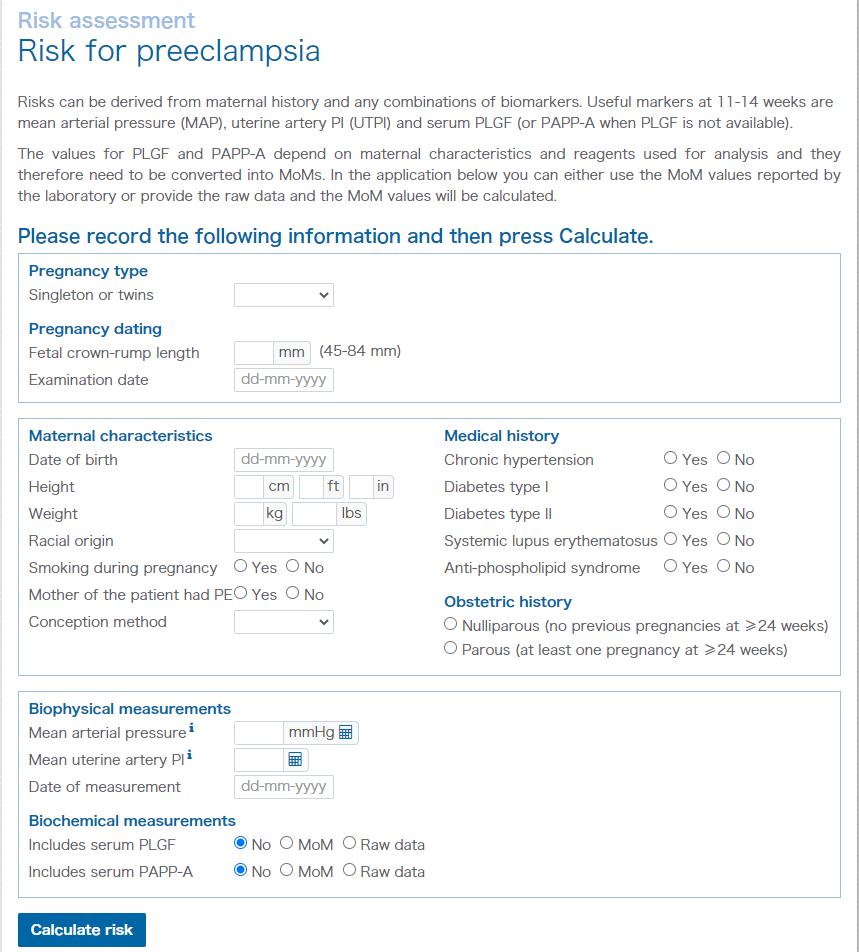
\includegraphics[width=.6\linewidth]{ch1/risk}
    \caption{\label{fig:risk}子痫前期风险因子评估量表}
\end{figure}

1. 产妇年龄

有证据显示,高龄孕妇(分娩时年龄超过35周岁)发生子痫前期的可能将增加1.2-3倍;当孕妇年龄大于35周岁时,其发生子痫可能增加;当年龄超过40周岁时,其发生子痫前期的可能将
增加两倍\cite{Duckitt2005,FIGO,Yogev2010}。
多项研究评估了子痫前期与孕妇年龄的风险,多元回归分析统计显示,当孕妇年龄超过32周岁时,孕妇年龄每增加1年,其发生子痫的可能增加4\%;当孕妇年龄超过34岁时,这一数值将激增至30\%。
但孕妇的年龄与其增加发生原发子痫前期的可能无关,即使年轻的孕妇仍有可能发生子痫前期\cite{Duckitt2005,Poon2010}。

2. 胎产次

临床统计发现,初产孕妇患子痫前期的可能会增加。多项人口统计显示,这一感染风险甚至能达到惊人的三倍以上\cite{Lee2000,Duckitt2005,Coonrod1995}。另外一项调查研究显示,
没有既往子痫前期病史的经产孕妇患子痫前期可能的风险会降低\cite{Robillard1993}。

3. 既往史

2009年,Sonia等人对1987年至2004年间的763 795名首次分娩的产妇的相关数据进行了分析统计,结果显示首次分娩产妇罹患子痫前期的概率比未患有子痫前期既往史的二胎孕妇风险更大\cite{Sonia2009}。
对已分娩的妇女而言,在以后的妊娠中发生子痫前期的风险则与既往子痫前期发病史有很大关联,二次妊娠中发生子痫前期的相对风险可提高7-10倍\cite{Duckitt2005,CAMPBELL1985,Lie1998,Sibai1986}。

4. 妊娠间隔

临床研究证实,多次妊娠间隔时间过长或过短都会在一定程度上增加PE发生的风险\cite{Rousso2002,Duckitt2005,Conde2007}。2016年,Mignini等人\cite{Mignini2016}对拉丁美洲1990年-2009年间的894 479名孕妇进行了统计
分析,结果显示与孕妇二次妊娠间隔12-23个月相比,妊娠间隔不到12个月或超过72个月则会增加PE患病风险。Rolv\cite{Rolv2002}等人对挪威的551 478名多次妊娠孕妇的研究调查显示PE既往史对孕妇二次妊娠具有短暂
的保护作用,孕妇二次妊娠的PE患病风险与上次分娩后经过的时间直接相关。

5. 辅助生殖

多项临床研究显示,当孕妇通过辅助生殖技术(assisted reproductive technologies,ART)受孕时,其PE患病可能会增加一倍\cite{Jackson2004,Trogstad2009}。 Angela S. Martin等人\cite{Martin2016}的研究显示,
不论通过何种具体ART受孕的孕妇与自然受孕的孕妇相比,其患子痫前期的风险均有所增加。这一结果可能ART过程中雌激素水平过高可能导致胎盘受损和子宫胎盘循环减少以及子宫螺旋动脉血管浸润的减少有关。

6. 家族史

临床研究统计显示,PE在一定程度上显现出家族性易感性\cite{ARNGRIMSSON1990,OAG9,Williams2011}。(曾)患有PE的女性的女儿或姐妹发展成PE的可能性是没有家族PE史的女性的3-4倍\cite{ARNGRIMSSON1990,Cincotta1998,FIGO,Williams2011}。但PE具体遗传方式与机制尚不明确。

7. 肥胖

多项临床统计表明,若孕妇出现肥胖症状($BMI>30kg/m^2$),则其PE患病可能会增加2-4倍\cite{Williams2011,FIGO,Zintzaras2006}。但肥胖与PE的具体作用机制尚不清楚。另一方面,由于出现肥胖的孕妇往往是高龄孕妇,其患慢性高血压的可能也较大。但排除掉这些因素可能的影响,
肥胖仍然会导致PE患病风险增加\cite{Duckitt2005}。另一方面,Sebire等人\cite{Sebire2001}在2001年的一项研究表明,当孕妇BMI指数<20时,其PE风险显著降低,则从侧面验证了肥胖对PE的影响。

8. 种族

人口统计研究表明,不同民族、区域、肤色的孕妇其子痫患病可能会有一定的差异\cite{Ghosh2014,Khalil2013}。

9. 并发症

当孕妇自身已患有某些疾病或感染某些症状时,其PE患病可能也会增加\cite{FIGO,Ray2016,OAG9}。临床研究已证实,这些疾病包括胰岛素依赖型糖尿病\cite{Lee2000,Garner1990}、肾病\cite{Martinell1990}、
慢性自身免疫病\cite{Stamilio2000}及抗磷脂综合症\cite{Dreyfus2001,Marchetti2016}等。

% \begin{table}[htbp]
%     \centering
%     \fontsize{10}{6}
%     \caption{\label{tab:complication}可能引发PE的长短期并发症}
%     \begin{tabularx}{\linewidth}{cX<{\centering}}
%         \toprule \textbf{短期并发症}&\textbf{长期并发症}\\
%         \midrule 
%         胎儿生长受限&脑瘫\\
%         羊水过少&低智商\\
        
%         \bottomrule
%     \end{tabularx}
% \end{table}

庄彩霞等人\cite{Zhuang2019}对中国境内的98 000余例分娩孕妇进行了分析,得出了中国人群子痫前期的主要独立风险因子包括:慢性高血压疾病、既往子痫前期病史、$BMI≥28kg/m^2$、肾脏疾病、多胎妊娠、心脏病、$BMI 24~28kg/m^2$等。

二、生物标志物筛查

筛查PE的另一种方法是基于贝叶斯定理,将单个孕妇的PE风险因子和及其母体特征病史的先验风险与其进行的各项生物物理、生物化学检测结果相结合,从而估计其PE患病风险\cite{FIGO}。这一过程即为参数估计中的极大后验概率估计
(maximum a posterori,MAP),即按照观测值判断当前值x最可能属于哪一类进行分类决策\cite{TJXHCL}。不失一般性,以二元检测问题为例,MAP分类过程可以表示为
\begin{equation}
    \label{equ:maxap}
    H_{x}=
    \left \{
    \begin{aligned}
        &H_{1}, \text P(H_{1}|x)&>P(H_{0}|x), \\
        &H_{1}, \text P(H_{1}|x)&<P(H_{0}|x),
    \end{aligned}
    \right.  
\end{equation}
其中,$P(H|x)$为观测值x属于$H$的后验概率,选出从观测值x所有类别中选出后验概率最大的,即为观测值所属类别。上述筛选过程9中孕妇的生理、生化检测结果统称为生物标志物(biomarker),生理参数主要包括血压、子宫动脉搏动指数等,生化参数
(biomarker)则种类繁多、新参数层出不穷\cite{Rene2008,Zhong2015,Zeisler2016,Rana2012},这里选取血清妊娠相关蛋白A(Pregnancy associated plasma protein A,PAPP-A)与血清胎盘成长因子(placental growth factor,PLGF)为代表进行介绍。

1. 血压

由于PE是妊娠期高血压疾病的一种\cite{OAG9,HDASOM,2000s1},血压对PE的影响和意义不言而喻。血压值一直以来是临床用以对PE监测、诊断的重要指标。测量血压时,孕妇同一手臂应至少测量两次,收缩压>140mmhg和或舒张压>90mmhg定义为高血压。
对首次发现血压身高的孕妇,应至少间隔4小时后再次测量确认\cite{OAG9}。除基本的收缩压(systolic blood pressure,SBP)、
舒张压(diastolic blood pressure,DBP)外,平均动脉压(mean arterial pressure,MAP)更是作为国际妇产科联盟的建议指标,用于实际标定诊断PE之中,其计算方法如\autoref{equ:map}所示\cite{FIGO}。
\begin{equation}
    \label{equ:map}
    MAP=DBP+(SBP-DBP)/3
\end{equation}
Leona C.Y. Poon\cite{Poon2008}等人对5590名单胎孕妇的一项研究表明,当单独使用MAP进行检测时,PE的检测率为38\%;当结合孕妇病史等因素时,PE检出率可达63\%,假阳性率为10\%。
Stamilio等人\cite{Stamilio2000}发现,孕妇第一次产前检查时出现MAP>90毫米汞柱与其PE患病的可能相关性显著。

2. 子宫动脉搏动指数

UTPI是国际妇产科联盟与妇产科超声学会所推荐的对PE进行筛查的参数之一\cite{FIGO,Sotiriadis2019}。\autoref{fig:utpi}展示了一例孕早期经腹多普勒超声检查子宫动脉的结果\cite{Sotiriadis2019}。
UTPI本质上也是一种血液动力学参数,其基本定义与MAP类似,是子宫动脉收缩期峰值流量$A$减去舒张末期流量$B$除以平均流量$M$\cite{Cnossen2008}:
\begin{equation}
    \label{equ:utpi}
    UTPI=\frac{A-B}{M}
\end{equation}
同时,常与UTPI一起检测的还有子宫动阻力动指数(Resistance index,RI)、子宫动脉(peak systolic to late diastolic ratio,S/D R)及切迹等参数\cite{Cnossen2008}。
\begin{figure}[htbp]
    \centering
    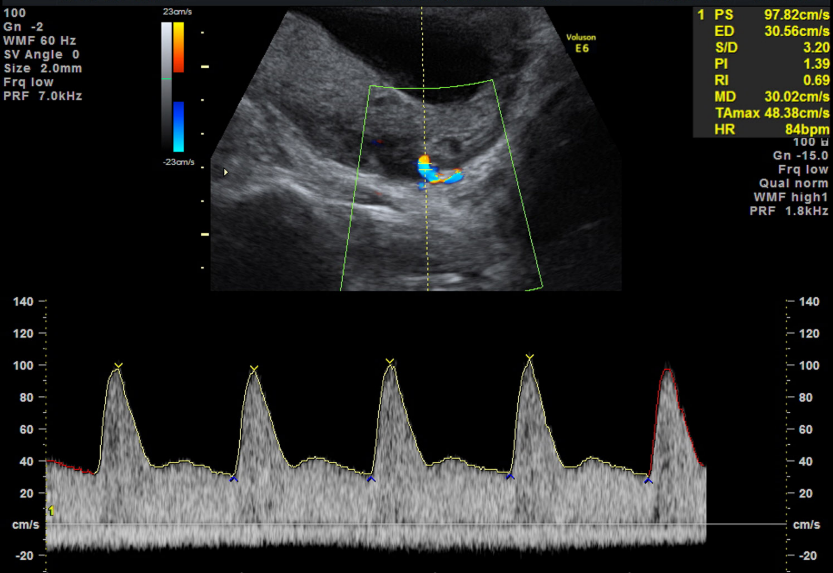
\includegraphics[width=.6\linewidth]{ch1/utpi}
    \caption{\label{fig:utpi}孕早期经腹多普勒超声检查子宫动脉}
\end{figure}
Jeltsje S. Cnossen等人\cite{Cnossen2008}此前众多学者研究的回顾表明,在孕妇妊娠$11^{+0}-13^{+6}$周时,若子宫动脉多普勒血流检测发现UTPI上升或出现子宫动脉舒张早期切迹等印象,则该孕妇PE患病的可能将增加\cite{OAG9,Plasencia2008}。

3.血清妊娠相关蛋白A

PAPP-A是由细胞滋养层分泌的一种金属蛋白胰岛素生长因子结合蛋白,在胎盘的生长发育中起着重要的作用。PE已被证明与低水平的PAPP-A循环有关\cite{FIGO}。但相关临床研究表明,仅使用PAPP-A单指标无法准确预测PE\cite{Smith2002}。
因此,PAPP-A常与其他检测参数一起配合使用\cite{Poon2009,Tan2018,Ray2018}。 

4. 胎盘生长因子

PLGF是由绒毛状细胞滋养层膜细胞滋养层合成,是一种糖基化二聚糖蛋白,具有血管生成合血管修复的功能。临床研究显示,PLGF的血管生成功能在妊娠过程中会发挥很大作用,PLGF水平或其抑制受体水平的变化可能与PE的发生有关\cite{Levine2004,Ahmad2004}。
同时,临床证据表明,在孕早期患有PE的孕妇其PLGF的浓度较正常妊娠孕妇更低\cite{Chau2017}。
2019年,Duhig等人\cite{Duhig2019}对1019名疑似PE的孕妇进行了追踪实验,在整个实验期间一直持续性的进行PLGF水平检测。结果显示,针对实验组(n=573),PE诊断时间的中位数为4.1天,而对照组(n=446)这一数值仅为1.9天,证明PLGF可以有效的缩短PE确诊的时间。
2015年,Zhong等人\cite{Zhong2015}对多项血清生化指标在PE预测方面的性能进行了比较,结果显示,PLGF的综合性能优于其他诸如胎盘蛋白13(Plancenta protein 13,PP13)、PAPP-A
等其他血清生化指标。鉴于此,\textbf{FIGO组织特别将胎盘生长因子推荐为PE检测首选生化指标}\cite{FIGO}。

\subsection{分析及检测设备}
一、标准医疗设备

目前临床所使用的PE筛查检测设备主要以检测生化标志物为主,国内外医疗器械公司研发推出了一系列软硬件综合分析系统。但整体而言,国内医疗器械设备公司研发起步晚,检测指标较国外设备数目少。

1. 德国勃拉姆斯公司的产前检测设备

勃拉姆斯公司(B·R·A·H·M·S GmbH)一直致力于对各种生物标志物检测的研究中,其公司产品KRYPTOR GOLD与KRYPTOR compact PLUS\cite{B·R·A·H·M·S2021}可完成对AFP、Free $\beta$hCG、$\beta$hCG、PAPP-A、PlGF、
sFlt-1、uE3等在内的多种生物标志物的检测,
满足PE的早期筛查及诊断等多种应用场景,如\autoref{fig:B·R·A·H·M·S}所示。同时该公司还研发了一套Fast Screen pre I plus$^\text{TM}$综合软件分析系统,可结合检测结果对孕妇PE发病可能进行风险评估。

\begin{figure}[htbp]
    \centering
    \subfigure[KRYPTOR GOLD]{
    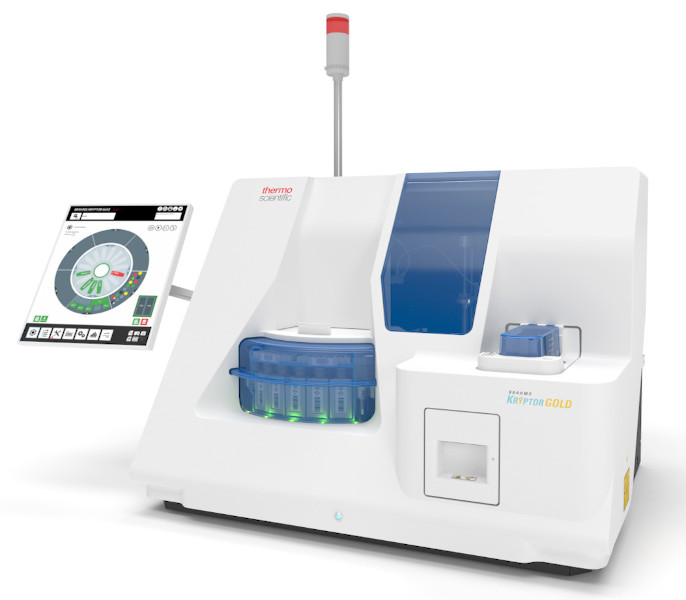
\includegraphics[width=5.5cm]{ch1/brahms-kryptor-gold-686}
    }
    \quad
    \subfigure[KRYPTOR compact PLUS]{
    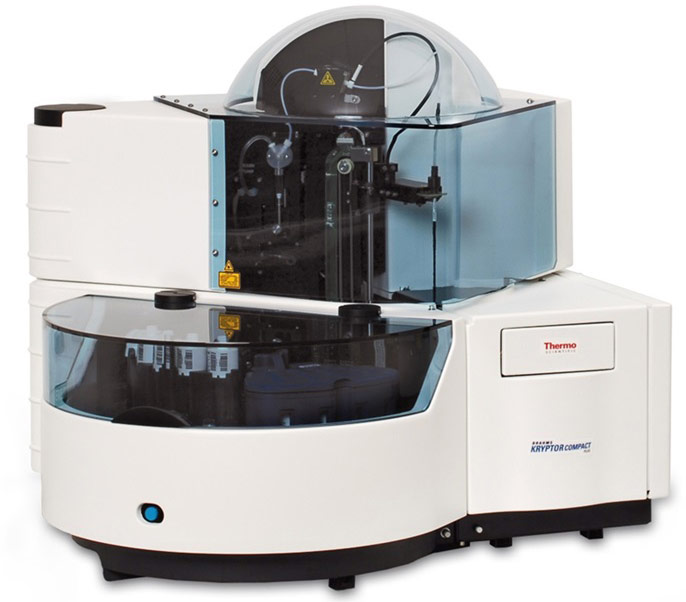
\includegraphics[width=5.5cm]{ch1/brahms-kryptor-compact-plus-686}
    }
    \caption{\label{fig:B·R·A·H·M·S}勃拉姆斯公司KRYPTOR系列的两款检测设备}
\end{figure}
2.美国珀金埃尔默公司的产前检测设备

珀金埃尔默公司(PerkinElmer)提供全面的筛查和诊断解决方案组合,推进早期临床检测在成医疗领域的应用。该公司针对PE在内的多种孕期综合并发症提出了完整的检测方案,其AutoDELFIA系列、
VICTOR2系列及DELFIA Xpress系列的多款免疫荧光分析仪平台\cite{perkinelmer2021}均可完成对AFP、Free $\beta$hCG、$\beta$hCG、PAPP-A、PlGF、
sFlt-1、uE3等在内的PE生物标志物检测标定,如\autoref{fig:PerkinElmer}所示。此外,该公司位硬件检测设备配套研发了LifeCycle软件分析系统,实现了从样品接收-检验检测-风险评估-化验报告的全自动工作流程。
\begin{figure}[h]
    \centering
    \subfigure[VICTOR2 D荧光检测仪]{
    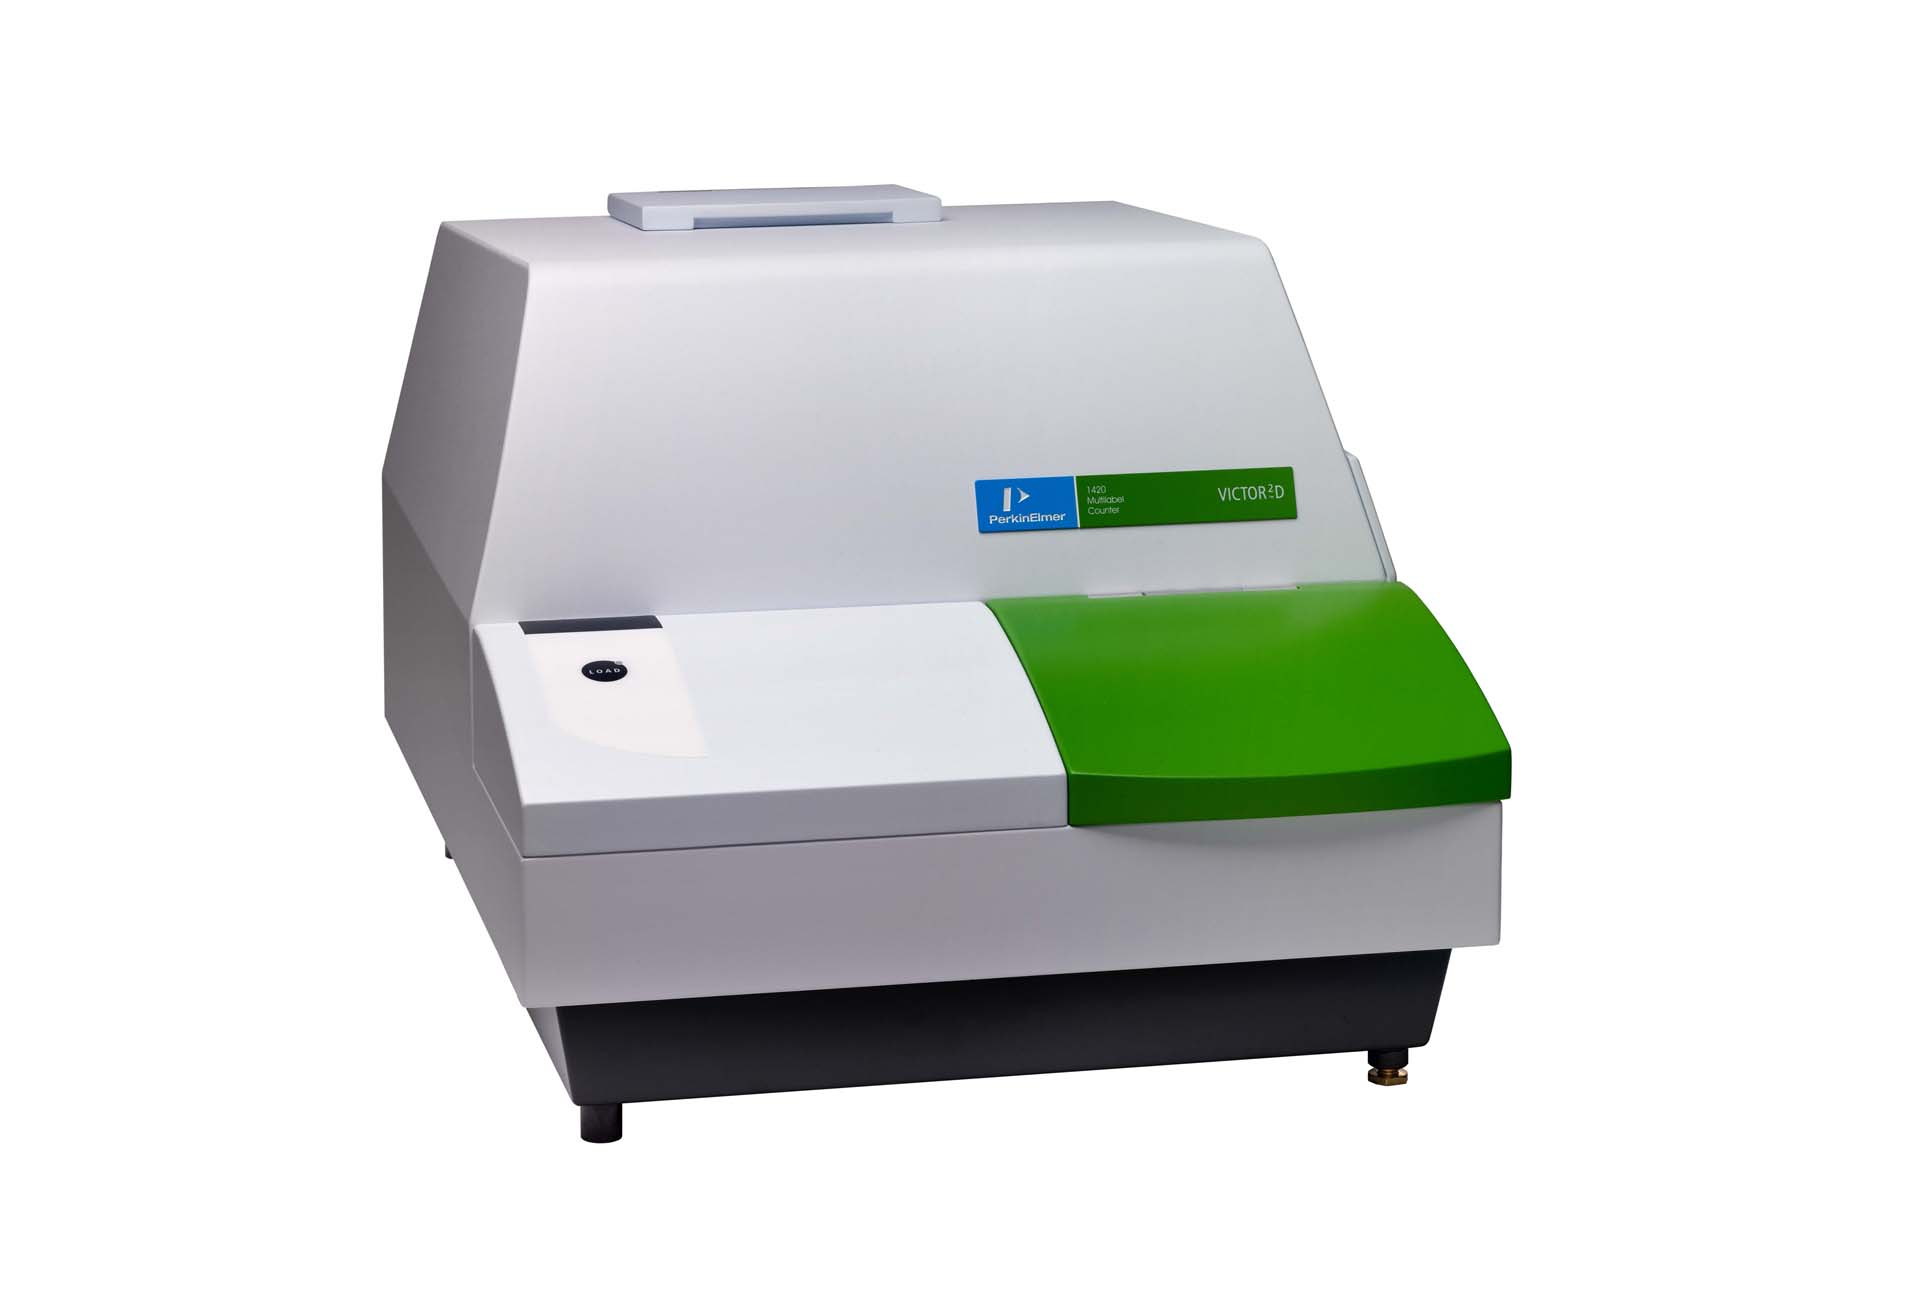
\includegraphics[width=5.5cm]{ch1/Victor-2D-72ppi}
    }
    \quad
    \subfigure[DELFIA® Xpress免疫分析仪平台]{
    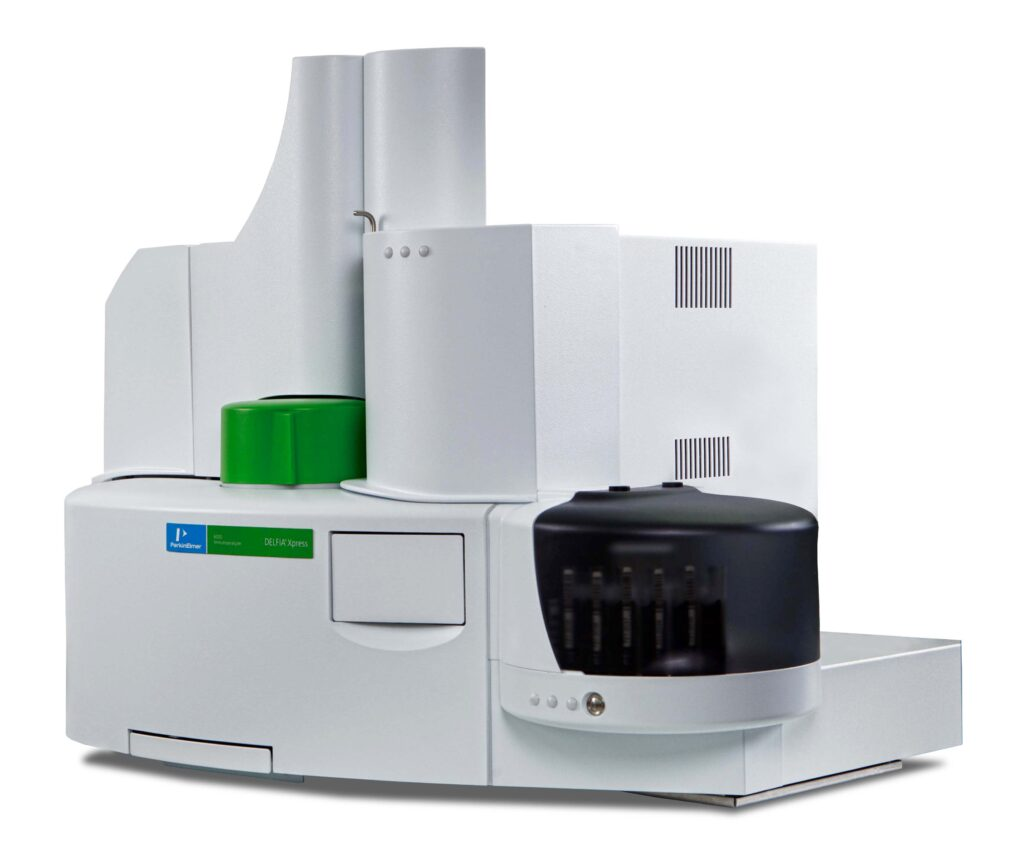
\includegraphics[width=5.5cm]{ch1/dx}
    }
    \caption{\label{fig:PerkinElmer}珀金埃尔默公司的两款检测设备}
\end{figure}

3. 中国宁波奥丞生物科技有限公司的荧光检测设备

作为中国新兴的医疗器械设备公司,奥丞专注于从疾病早期发现、诊断、预防到监测,力求通过提供可靠、快速与便捷的体外诊断产品为诊疗提供精准的检测结果。
目前,奥丞公司的多款化学荧光免疫平台产品均支持对PE生物标记物PLGF、sFlt-1等两种指标的检测\cite{aucheer2021}。此外,奥丞还根据实际临床需求,
提供了微小型床边诊断设备与大型实验室标定两种类型的设备,如\autoref{fig:aucheer}所示。
\begin{figure}[h]
    \centering
    \subfigure[微流控荧光免疫定量检测系统 iSort300]{
    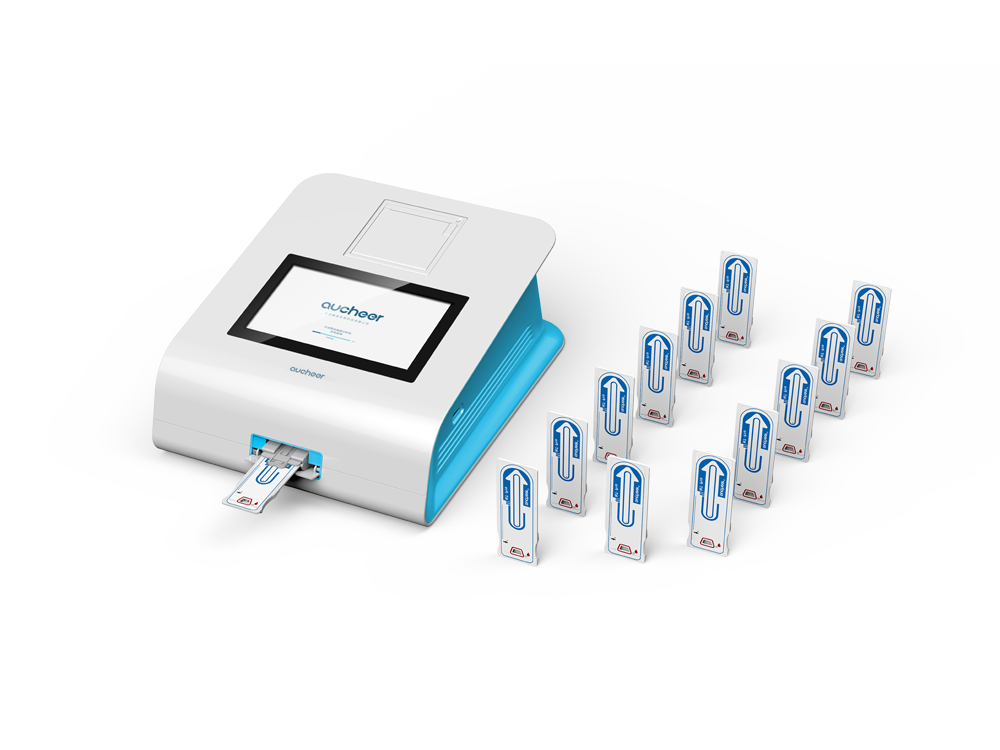
\includegraphics[width=5.5cm]{ch1/isort300}
    }
    \quad
    \subfigure[全自动化学发光免疫检测系统 Shine i1910]{
    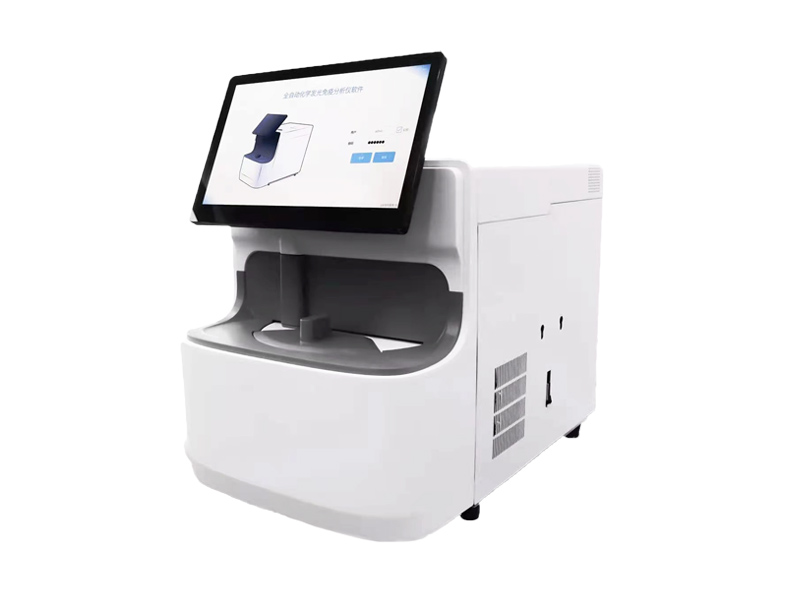
\includegraphics[width=5.5cm]{ch1/shinei1910}
    }
    \caption{\label{fig:aucheer}奥丞生物科技公司的荧光免疫平台}
\end{figure}


二、微型智能设备

随着移动智能医疗和可穿戴式设备的发展,通过微型智能设备实现对PE相关指标的实时、动态、多场景检测也逐渐成为了新的研究热点。但整体而言,基于智能设备的PE检测设备仍处于研发阶段,能真正实现多场景检测的成熟的PE分析系统尚未出现。
2019年,Iuliana Marin等人\cite{Marin2019,Marin2020}通过一款智能腕部血压检测穿戴设备对孕妇的血压数据进行了监测,同时综合考虑孕妇的年龄、体重等风险因素,通过维特比动态规划算法(Viterbi algorithm),判断决策孕妇子痫前期
的患病可能,该系统原理框架图如所示。Iuliana Marin团队
通过对105名试验人员进行了测试,结果显示,最终的生成模型可以达到总体准确率80\%,敏感性为92.5\%,特异性为72\%\cite{Marin2019}。
\begin{figure}[htbp]
    \centering
    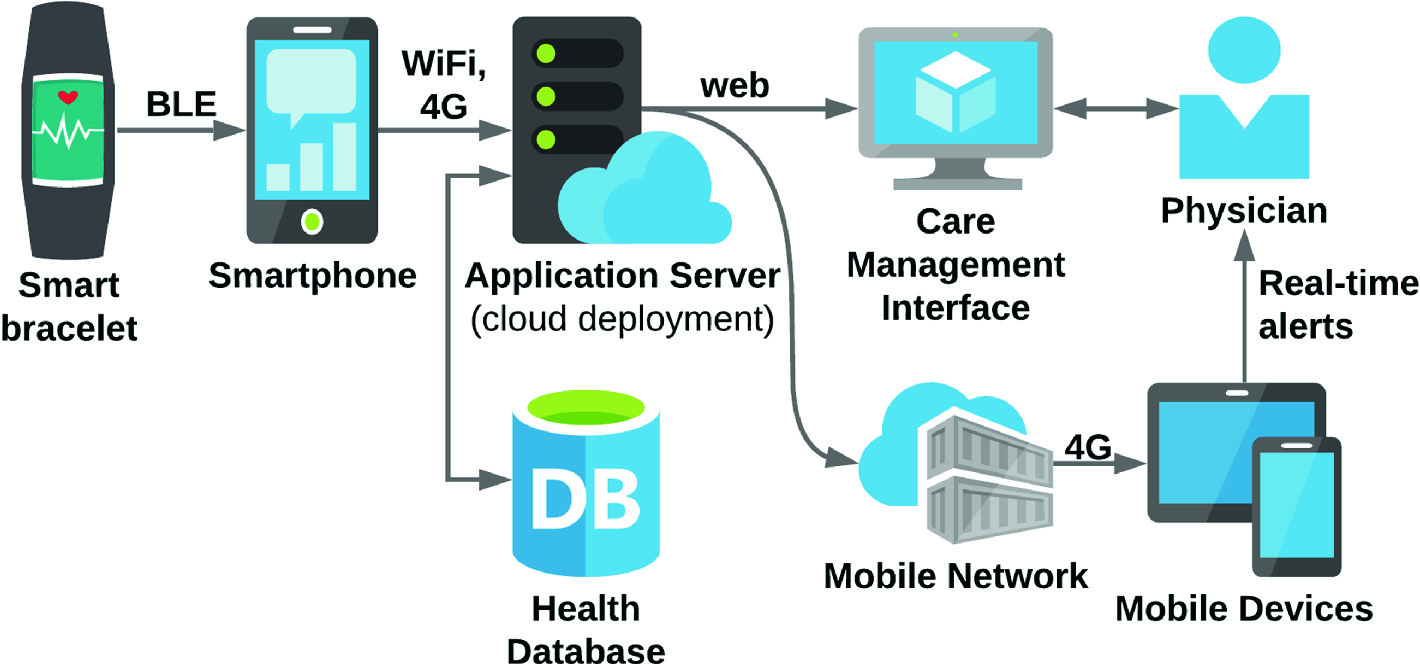
\includegraphics[width=.6\linewidth]{ch1/mobile}
    \caption{\label{fig:mobile}基于智能穿戴设备的血压检测系统框架图}
\end{figure}

\subsection{分析技术}
近年来,由于现代化设备的普遍使用致使医学检查过程各项数据激增,同时计算机领域人工智能技术的不断创新发展,相关研究者也开始尝试在子痫前期的识别、判断乃至预测等研究内容上引入人工智能技术。
利用人工智能技术分析前小节提到的各项风险因子、生理化学等参数一时间成为了炽手可热的多学科交叉研究点。
2016年,Rutvij Mehtad等\cite{Mehta2016}将大数据挖掘技术(Major Data Mining)在预测子痫前期、产科风险因素及产科其他疾病等健康领域的主要研究进行了归纳总结。他们将诸多学者的研究涉及的
数据挖掘与分析总结为两大类应用研究方向,即关联规则(Association Rule)挖掘方向与分类、聚类分析方向。关联规则挖掘力求发现多项数据之间的隐藏的逻辑与关系;分类分析是对通过现有数据建立模型预测新数据所属类别,
聚类分析则是按照一定规则将所有数据分组,使每组内的数据尽可能相似并有别于其他组数据\cite{Han2006}。在两大类应用的基础上,学者们使用不同的数据对子痫前期进行了分析研究。

一、数据挖掘

从众多的原始数据中筛选出与研究问题最为相关的部分,在实现数据降维的同时发现数据之间隐藏的联系是数据挖掘技术重要的研究内容。
如何从血浆代谢物、蛋白质及$mRNA$等生化指标中筛选出与PE患病最为相关的成份,此前的学者们也做了很多研究。

2005年,Louise C. Kenny等人\cite{Kenny2005}从利用基因遗传算法(genetic programming,GP),从血浆中代谢物成份确定特异的成份来识别患有PE的孕妇。他们通过对受试孕妇(其中,患有PE的实验组$N_{PE}=87$,正常对照组$N_{Normal}=87$,下同)
的血浆成份分析后,通过GP训练出了仅使用三种代谢物峰值变量预测模型。预测模型可以有效区分患有PE与正常孕妇,其灵敏度高达100\%,特异性高达98\%。

2020年,Jose F Carre˜no等人\cite{Carreno2020}基于蛋白质组学数据,改进了基于比较的特征选择算法进行了子痫前期的预测。特征算法包括帝国竞争与基因集簇两种降维算法与三点时间序列(分别对应孕前中晚期数据)总结算法两方面。
改进后的方法在两个独立数据集上均有90\%左右(85\%-93\%)的准确性,同时结果显示,孕早期与孕中期的蛋白质组学数据用以子痫前期的预测相较孕晚期结果会更准确。

2018年,Liron Yoffe等人\cite{Yoffe2018}对怀孕前三个月孕妇血浆中非编码循环RNA的丰度进行了分析,寻找能有效区分识别PE的转录RNA。他们在对孕妇的非编码RNA测序后,确定了实验组与对照组($N_{PE}=75$,$N_{Normal}=75$)
之间差异表达的25个RNA,最终训练生成了一个逻辑回归模型,经五层交叉验证,模型的AUC高达0.86。

同样是对RNA的研究,2021年Rong Guo等人\cite{Guo2021}则是利用集成学习投票决策算法筛选能够识别PE的胎盘mRNA。在获取了原始数据($N_{PE}=157$,$N_{Normal}=173$)后,他们基于相关性完成了数据降维,仅保留了原始48个差异表达基因中的13个。
同时通过构建了C4.5决策树(decision tree, DT)、自适应增强(adaptive boost, AdaBoost)及多层感知机(multilayer perceptron,MLP)三种分类器并通过多数投票策略,他们将分类识别准确性从开始的$79\%$提高至$82.2\%$。

2018年,Muhlis Tahir等人\cite{Tahir2018,Tahir2018-2}对比了利用神经网络和深度学习两种算法预测妊娠期孕妇PE的风险水平的结果。他们使用粒子群优化(PSO)作为特征选择算法,将原始数据集(n=1077)的17个参数降维至9个。
在原始数据上通过LOO验证表明,深度学习后的模型具有95.12\%的准确率,使用经过缩减的数据集准确性还可提升至95.68\%。而当使用神经网络算法时,算法准确性亦可高达96.66\%。

二、 分类分析与聚类分析

所谓分类(Classification),就是按照某种标准给对象贴标签(label),再根据标签来区分归类;而聚类,则是在是指事先没有“标签”的情况下,通过某种聚集分析,找出事物之间存在聚集性原因的过程。分类分析与聚类分析是PE在机器学习领域最活跃的方向,而前文
提到的PE风险因子则是最为广泛使用的基础数据。

2017年,Pia M. Villa等人\cite{Villa2017}通过贝叶斯聚类算法,对受试孕妇(N=903)依据PE风险因子进行了聚类分析,对聚类结果分别计算了其PE患病可能。其聚类分析的热力度如\cite{fig:Heatmap}所示。
结果PE的患病可能随孕妇具有的PE风险因子数量呈指数增长;同时,不同程度的PE往往其风险因子种类也有不同。
\begin{figure}[htbp]
    \centering
    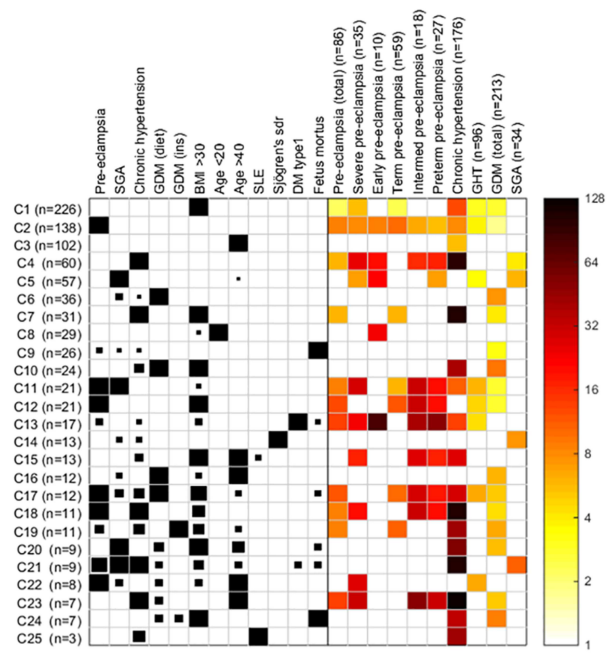
\includegraphics[width=.6\linewidth]{ch1/heatmap}
    \caption{\label{fig:Heatmap}热力图}
\end{figure}

2020年,Oknalita Simbolon等人\cite{Simbolon2020}基于软投票的集成学习算法,利用多项PE风险因子数据为PE患病高危孕妇开发了一款具有PE预测与推荐建议的智能手机APP。智能APP通过K近邻、线性支持向量机、RBF支持向量机、高斯过程、多层感知器和Ada-Boost等
6个单独的分类器分别对孕妇的PE患病可能进行预测,最后通过软投票的方法得出最佳预测模型并以此为孕妇给出相应的意见。通过对402的孕妇的数据测试表明,使用该算法最后能得到98.51\%±0.0186\%的高精度值,整体表现胜过其中任一单独分类器。

2011年,EDUARDO TEJERA等人\cite{Tejera2011}通过人工神经网络(Artificial neural network,ANN)完成了可对不同胎龄的正常孕妇、高血压孕妇及PE孕妇进行分类的模型构建。他们将\textbf{从ECG记录中获取的孕妇连续RR间期}(n=568)与孕妇病史、血压值等其他风险因子结合作为模型输入。
最终训练所得的模型对PE识别的敏感性约为80\%,特异性约为85\%。

2020年,Ivana Mari{\'{c}}\cite{Maric2020}等人借助统计学习中的弹性网算法(Elastic Net Algorithm,ENA)从诸多可能导致子痫前期的风险因子等变量中训练了预测模型。经验证,该预测模型对子痫前期的预测ROC数值可以0.79,准确度可达45.2\%;模型对早发子痫前期预测的
ROC高达0.89,此时真阳性为72.3\%,假阳性为8.8\%。

2020年,Herdiantri Sufriyana等人\cite{Sufriyana2020-1}基于PE风险因子及生化指标(包括sFlt-1、UPTI与PlGF)对孕妇($N_{PE}=66$,$N_{Normal}=29$)PE发生情况进行了研究。经过特征筛选、多种模型性能对比,
他们最终通过M5P树状回归演算法训练获取的模型具有最佳分类效果,可实现100\%的精确度与95\%的敏感度。研究同时发现,最佳模型的特征是孕妇体重、BMI、UPTI、sFlt-1和PlGF,尤其是sFlt-1/PlGF比值。
同年,Sufriyana团队进行的另外一项研究\cite{Sufriyana2020}则聚焦于与PE相关的特征。他们对包含95个特征的印度尼西亚孕妇数据集($N_{PE}=3318$,$N_{Normal}=19883$)进行了建模分析。经筛选,最终由17项特征生成的随机森林模型对PE具有
最好的预测分析效果。

综上,基于机器学习的PE研究可总结为表所示,由于篇幅内容所限,一些正文里未做介绍的额外研究也在表中进行了补充。
\begin{table}[hp]
    \centering
    \fontsize{10}{6}
    \caption{\label{tab:test}示例表格}
    \begin{tabularx}{\linewidth}{cX<{\centering}X<{\centering}X<{\centering}X<{\centering}X<{\centering}}
        \toprule \textbf{类型}&\textbf{研究者}&\textbf{机器学习方法}&\textbf{主要涉及指标}&\textbf{数据}&\textbf{研究结果}\\
        \midrule PE&preeclampsia&子痫前期,先兆子痫\\
        HDP&hypertension disorders of pregnancy&妊娠期高血压疾病\\
        RF&random forest&随机森林\\
        SVM&support vector machine&支持向量机\\
        MLP&multilayer perceptron&多层感知机\\
        \bottomrule
    \end{tabularx}
\end{table}



% 2009年,-许多神经网络方案\cite{Neocleous2009}已应用于孕妇的大型数据库,旨在生成早期子痫前期发生风险估计的预测因子。该数据库由英国6838例孕妇组成,由伦敦Har-ris胎儿医学出生权研究中心提供。
% 对于每个受试者,测量或记录了24个参数。其中,15个参数被认为是表征先兆子痫发生风险的最重要参数。尝试了一些前馈神经结构,包括标准多层和多层板,用于预测。
% 获得的最佳结果是使用多板神经结构。在训练集中,83.6\%的先兆子痫病例分类正确,而在测试集中,分类正确率为93.8\%。完全未知验证试验对先兆子痫病例的预测为100\%


% 2019年,摘要\cite{Jhee2019}
% 本研究旨在利用医院电子病历数据,开发利用机器学习预测晚发性先兆子痫的模型。
% 还比较了基于机器学习的模型和使用传统统计方法的模型的性能。共有11006名孕妇在延世大学医院接受产前护理。
% 从电子病历中检索孕中期至34周期间的产妇数据。预测结果为妊娠34周后发生晚发性先兆子痫。
% 模式识别和聚类分析用于选择预测模型中包含的参数。采用Logistic回归、决策树模型、朴素贝叶斯分类、支持向量机、随机森林算法和随机梯度推进法构建预测模型。C-统计用于评估每个模型的性能。
% 总的先兆子痫发生率为4.7\%(474名患者)。收缩压、血清尿素氮和肌酐水平、血小板计数、血清钾水平、白细胞计数、血清钙水平和尿蛋白是预测模型中最有影响的变量。决策树模型、naïve Bayes分类、
% 支持向量机、随机森林算法、随机梯度推进法和逻辑回归模型的C-统计分别为0.857、0.776、0.573、0.894、0.924和0.806。随机梯度推进模型的预测性能最好,准确率和假阳性率分别为0.973和0.009。结
% 合使用母亲因素和从中期妊娠早期到晚期妊娠早期的常见触角实验室数据,可以使用机器学习算法有效预测晚发性先兆子痫。未来的前瞻性研究需要验证这些算法的临床适用性。


% 2018年,Antonieta Martínez-Velasco等人\cite{Martinez2018}通过基于子痫前期患病可能风险因子的数据库,进行了特征筛选、阈值优化等操作,训练并改进了基于监督学习的子痫前期预测模型,同时,利用决策树算法对模型进行可视化操作。
% 数据集包含1634条记录,每条记录包含25个数据特征。


% 在医学领域,\cite{Moreira2016}存在处理大量信息的不同情况,需要进行彻底的评估,以便能够在决策过程中帮助专家。智能决策支持系统允许对所有现有信息进行分组,并从中找到相关信息。
% 贝叶斯网络提供了允许信息捕获和处理不确定性情况的模型。本文提出了一个系统的建设,以支持智能决策应用于诊断先兆子痫贝叶斯网络,以帮助专家在怀孕的护理。还介绍了网络构造的定性和定量建模过程。
% 这项工作的主要贡献包括介绍一个贝叶斯网络,该网络用于帮助决策者在护理孕妇的不确定时刻提供帮助。


% 基因微阵列分析\cite{Nair2018}




% \begin{sidewaystable}[ph!]
% 	\begin{center}
% 		\caption{\label{tab:table5}Landscape table}
% 		\begin{tabular}{l|c|r}
% 			\toprule
% 			\textbf{value 1} & \textbf{value 2} & \textbf{value 3}\\
% 			\midrule
% 			1 & 1110.1 & a  \\
% 			\hline
% 			2 & 10.1    & b  \\
%             \hline
%             1 & 1110.1 & a  \\
% 			\hline
% 			2 & 10.1    & b  \\
%             \hline
%             1 & 1110.1 & a  \\
% 			\hline
% 			2 & 10.1    & b  \\
%             \hline
%             1 & 1110.1 & a  \\
% 			\hline
% 			2 & 10.1    & b  \\
%             \hline
%             1 & 1110.1 & a  \\
% 			\hline
% 			2 & 10.1    & b  \\
%             \hline
%             1 & 1110.1 & a  \\
% 			\hline
% 			2 & 10.1    & b  \\
%             \hline
%             1 & 1110.1 & a  \\
% 			\hline
% 			2 & 10.1    & b  \\
% 			\bottomrule
% 		\end{tabular}
% 	\end{center}
% \end{sidewaystable}


% \begin{figure}[htbp]
%     \centering
%     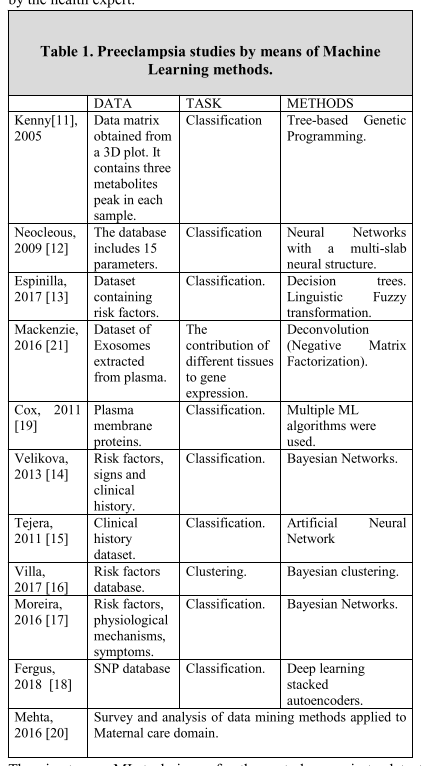
\includegraphics[width=.4\linewidth]{ch1/ai}
%     \caption{\label{fig:ai}部分对子痫前期的机器学习研究}
% \end{figure}

\subsection{存在的不足与分析}
综合上述分析,对子痫前期的早期识别与检测可从按以下思路开展深入探索与研究。


\section{脉搏波在子痫前期领域研究现状}
\subsection{用脉搏波检测子痫的优势}

\subsection{传统指标分析}

2008年,KARLIJN VOLLEBREGT等人\cite{KARLIJN2008}同时对223名孕妇的风险因子及指端脉搏波数据进行了分析研究,最终得到的子痫前期的预测模型具有较高的性能(ROC curve area 0.95, sensitivity 90\% and specificity 86\%),
其中,脉搏波参数AIx对模型具有很大的贡献度。

2012年,Kathleen Tomsin等人\cite{Tomsin2012}对静脉脉搏波传输时间参数(pulse transit time, PTT)进行了研究,结果显示除肝静脉和胸主动脉外,子痫前期的早期(n=12)及晚期患者(n=14)的PTT较正常孕妇(n=16)数值更低。

2014年,Ira Bernstein等\cite{Ira2014}人通过34名孕妇在孕早期(PRE)、12-14孕周(V2)及30-32孕周(V3)的手腕脉搏波PWV数据及心脏射血时间进行了测量与分析,结果发现子痫前期患者较正常孕妇,其PWV数值在V3期数值往往更大,
(pre- eclampsia: 0.121?0.113 vs. Controls: 0.139?0.132 secs; p¼.04)。

2017年,MIHAELA VIVIANA IVAN等人\cite{VivianaIvan2018}他们结合孕晚期的孕妇的脉搏波数据与其风险因子对子痫前期的患病可能进行了统计与预测。结果显示,PWV与孕妇的肌酐及
蛋白尿指标具有明显的正相关关系(r > 0.75, p < 0.001), and;同时他们发现当孕妇BMI数值>26时,其患子痫前期的可能明显提高。

2014年,Irene Katsipi等人\cite{Katsipi2014}也对脉搏波传播速度(Pulse Wave Velocity,PWV)在子痫前期的预测方面展开了研究。他们评估了孕妇的PWV数值、胎盘可溶性蛋白水平(sFlt-1)、血清尿酸水平以及24小时尿蛋白和钙排泄水平。他们的研究表明
PWV在这些标志物中有着最好的子痫前期预测能力,对子痫前期孕妇及有着81\%的检测率。在结合sFlt-1数值的条件下,检测准确率可进一步提高至90\%-92\%。

2018年,Kunyan Li等人

\subsection{创新指标}

2018年,Feng Jiang等人\cite{FengJiang2018,ChenH2019}基于光电容积脉搏波提出了一种新型形态学特征分层面积比(hierarchical area ratio,HAR)参数,通过HAR参数量化描述脉搏波下降支的下降趋势。通过对42例孕妇脉搏波数据的分析发现,HAR参数可对PE进行有效区分,
其中with an accuracy of 85.7\% and sensitivity of 100\%。

2018年,Ying Feng等人提出

2019年,陈婉琳等人\cite{Chen2019}基于光电容积脉搏波提出了光电容积斜率指数(photoplethysmography slope index,PSI),并通过对50例孕妇(子痫患者23例,正常孕妇27例)的脉搏波数据对PSI进行了检验,
结果表明其灵敏性和特异性分别达到 87.0\%和 96.3\%,准确性达到 92.0\%。

\section{研究目标与内容}

\subsection{研究目标}
综合应用各种方法,提取研发新型光电容积脉搏波形态学特征参数,构建一般通用的光电容积脉搏波的描述特征集合。在此基础上,通过特征筛选、压缩等算法提取出对子痫前期有一定甄别能力的特征集,
使用机器学习算法构建出子痫前期筛选识别模型,并对最终模型的性能表现进行验证评估。
\subsection{研究内容}
全文研究内容可分为数据源获取、信号预处理、特征参数提取与分析、子痫前期甄别模型训练构建及模型评估具体包括5个部分,如所示。每部分具体研究内容包括:
\begin{enumerate}
    \item 数据源获取。介绍本研究所采用的数据来源(临床现场采集),包括采集设备、采集流程及规范。  
    \item 信号预处理。对从硬件设备获取的PPG信号分析其信号成分特点,完成滤波去噪、去基线漂移、特征点检测及标准化等准备工作。
    \item 特征参数提取与分析。从脉搏波形态学等方面构建特征参数。
    \item 子痫前期甄别模型训练构建及评估。通过机器学习中的等方法构建子痫前期甄别模型,并验证模型准确性。
    \item 模型评估。
\end{enumerate}

\textbf{各章节的具体内容安排如下:}

第一章是绪论。介绍子痫前期的定义及危害,梳理了目前临床已应用的检测方法及指标,分析各项方法的缺陷与不足。最后确定提出了本文的研究目标与内容。

第二章是光电容积脉搏波概述。阐述了

第三章是光电容积脉搏波的特征点检测算法。

第四章是光电容积脉搏波的特征集构建。

第五章是基于光电容积脉搏波特征的子痫前期检测识别模型。通过等几种方法优化特征参数集并构建了子痫前期的甄别模型,通过等方面评估了各项模型的整体性能表现。

第六章是低耦合高拓展的软件综合分析系统的设计与实现。阐述了本研究包括数据源导入管理、预处理算法管理、特征拓展管理、标准数据管理、模型训练生成管理等方面在内的整体分析系统的软件设计思路,
介绍了为提高本研究各部分内的内聚性、降低各研究内容之间的耦合性、提高系统整体可拓展性及实用性、提高系统真正落地临床的可能性所做出的各项规划及实现。

第七章是总结与展望。对本论文的全部研究工作进行系统性总结,阐述本论文的创新工作点,并对下一阶段的研究工作内容进行了规划与展望。